% Appendix: at most 2 pages after the references. Sources: results/labels/,
% results/probes/binary_*_test.json, results/probes/synth_types_*.json,
% requirements.txt, configs/inference_synth_pilot*.yaml, README.md.
\section{Examples of the error labels}
\label{app:examples}

Examples from Qwen's labels, with the annotator's rationale paraphrased.
\cls{structural}: a pie chart with seven labelled sectors counted as six; the
adjacent 2017 bar reported for the asked 2018 bar. \cls{computation}: every input
printed and readable but the operation wrong, e.g.\ a ratio of levels (83/11)
where the question asks for a ratio of changes. \cls{not\_an\_error}: 0.95 for a
gold of 95\%, or a correct ratio 28/19 = 1.474 where the gold 1.18 matches no ratio
on the chart. \cls{ambiguous}: both gold and model wrong, or a question with
several readings that the model fits none of. \cls{fabrication} (Qwen's only
case): pie slices of 35, 40, 13 and 11, gold 75, model 55, which matches no slice
and no sum.

\section{Layer profiles}
\label{app:layers}

Figure~\ref{fig:binary} shows the binary probe by relative depth: the last
prompt token rises from about 0.70 at the first layer to a plateau over the last
third of each network (best at layer 21 of 28 for Qwen, 24 of 32 for LLaVA), while
image-token positions stay at 0.62 to 0.68, near the surface baseline. For chart
errors the informative state is the one that has read the question, unlike HALP's
finding for object hallucination \citep{kogilathota2026halp}.
Figure~\ref{fig:types} shows the synthetic type probes: the missing-bar signal
saturates early (Qwen by layer 3, LLaVA by about layer 8), the misread signal
builds gradually and peaks in the last third.

\begin{figure}[h]
\centering
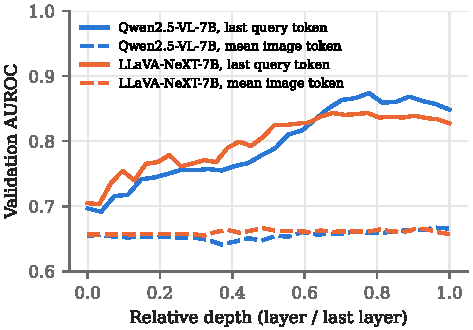
\includegraphics[width=\columnwidth]{figures/binary_by_layer.pdf}
\caption{E1 binary probe, validation AUROC by relative depth. Solid: last prompt
token; dashed: mean over image tokens.}
\label{fig:binary}
\end{figure}

\begin{figure}[h]
\centering
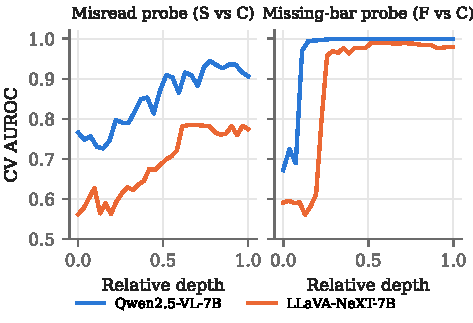
\includegraphics[width=\columnwidth]{figures/type_probes_by_layer.pdf}
\caption{Synthetic type probes, out-of-fold AUROC on their own task by relative
depth.}
\label{fig:types}
\end{figure}

\section{Reproducibility}
\label{app:repro}

All runs used RTX 2080 Ti GPUs in fp16 with SDPA attention, PyTorch 2.8.0,
Transformers 4.57.6 and seed 42, with greedy decoding of at most 32 new tokens;
the full environment is pinned in \texttt{requirements.txt}. Synthetic charts
are rendered with Matplotlib 3.10.0 and are deterministic given the seed; the
SHA-256 hashes of the three manifests (pilots 1 to 3) begin \texttt{20e80119},
\texttt{41fc27e5} and \texttt{ed311841}. Activations are pooled in fp16 and kept
off the repository. Every number in this report is read from a file in
\texttt{results/}, and the repository README lists the command that produces
each file.
